\section{QtDesigner: ¿C\'omo se usa?}
La idea principal de esta secci\'on es orientar en el uso de cada parte de la interfaz de QtDesigner, siguiendo
el desarrollo de algunos ejemplos simples que pueden encontrarse tambi\'en en la carpeta de ejemplos del \href{https://github.com/nicotrozzo/pyqt5-tutorials}{Repositorio de GitHub}.

\subsection{Creaci\'on de un Form} Abrimos QtDesigner, o en New File..,vamos a encontrar esta ventana. Nos deja crear
una nueva form de entre esas opciones. Tenemos que tener en mente que \textbf{Widget} ser\'a cualquier elemento dentro de una interfaz,
\textbf{Main Window} ser\'a una ventana principal que manejar\'a el flujo principal del programa, y \textbf{Dialog} es una ventana emergente (¡de hecho
esta ventana de QtDesigner es un Dialog!).


\begin{itemize}
    \item No deber\'iamos tener m\'as de un Main Window en nuestro proyecto.
    \item Siempre que creemos entre estas tres opciones, nuestra clase heredar\'a alguna de ellas. QWidget, QMainWindow o QDialog.
    \item Existen dialogs (QDialog) ya provistos por el framework, fijate despu\'es \nameref{dialogs_utiles}.
\end{itemize}

\begin{figure}[H]
    \centering
    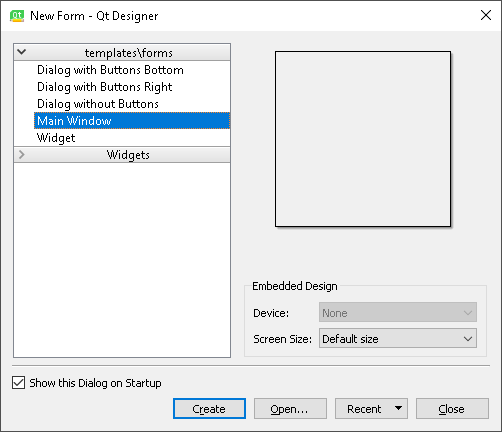
\includegraphics[scale=0.8]{imagenes/qtdesigner/qt_new_file.PNG}
    \caption{Ventana de creaci\'on de formas}
    \label{fig:qt_new_file}
\end{figure}

\subsection{¿Qu\'e es cada cosa en la IDE?}
Es importante conocer la organizaci\'on general de la IDE que estamos usando, saber de qu\'e es capaz puede ser un conocimiento
\'util para solucionar problemas f\'acilmente. En primer lugar veamos en la Fig. \ref{fig:qt_ide_0} algunas cosas elementales, la WidgetBox,
nuestro espacio de trabajo y dise\~no, y las opciones de Layout del Widget.

\begin{figure}[H]
    \centering
    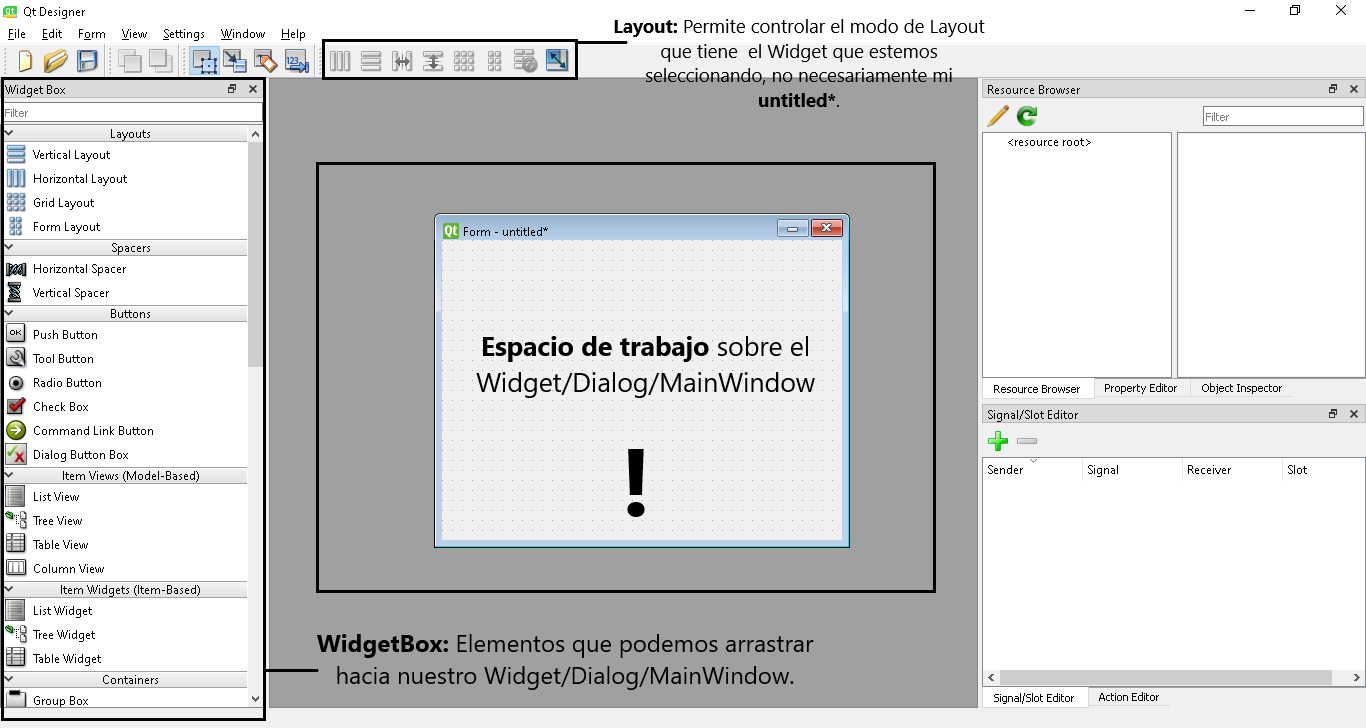
\includegraphics[scale=0.44]{imagenes/qtdesigner/qt_ide_0.png}
    \caption{Esquema inicial de la IDE}
    \label{fig:qt_ide_0}
\end{figure}

Ahora, para continuar con la descripci\'on del ejemplo vamos a hacer algunas cosas sencillas. Recordemos,
no importa no entender algunas cosas de c\'omo es PyQt, sino reconocer las partes de la IDE, por ahora...
Entonces agregamos un HorizontalSlider, un LCDNumber y luego aplicando un VerticalLayout, se obtiene esta Fig. \ref{fig:qt_ide_1}.

\begin{figure}[H]
    \centering
    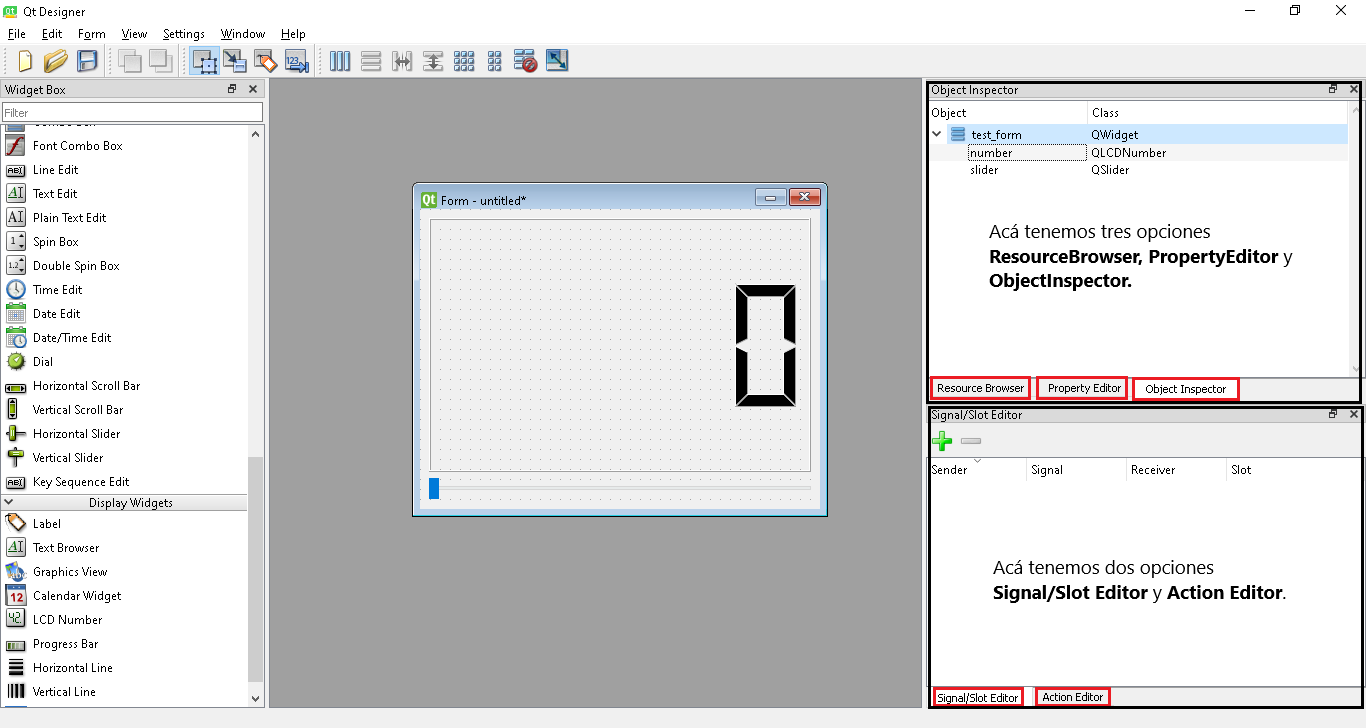
\includegraphics[scale=0.44]{imagenes/qtdesigner/qt_ide_1.png}
    \caption{Editores m\'as avanzados}
    \label{fig:qt_ide_1}
\end{figure}

\subsubsection{Object Inspector}
En PyQt existen tres elementos vamos a estar creando, que son el QWidget, QMainWindow y el QDialog. No obstante toda entidad que utilicemos hereda eventualmente
de un QWidget, y armar una ventana es poner QWidgets uno dentro de otros de forma organizada para armar nuestra aplicaci\'on, lo cual nos deber\'ia dejar la idea
de que internamente esto se comporta como un \'arbol, y el mismo se puede visualizar en el Object Inspector.
En el ejemplo vemos un QWidget, que internamente posee dos objetos y el campo \textbf{Object} es el nombre de la instancia durante ejecuci\'on,
con lo cual esto debe tener un nombre adecuado a la convenci\'on de Python de forma representativa.

\begin{figure}[H]
    \centering
    \begin{tabular}{c c}
        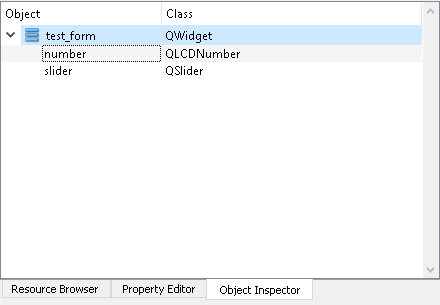
\includegraphics[scale=0.7]{imagenes/qtdesigner/qt_object_inspector.PNG} \\
        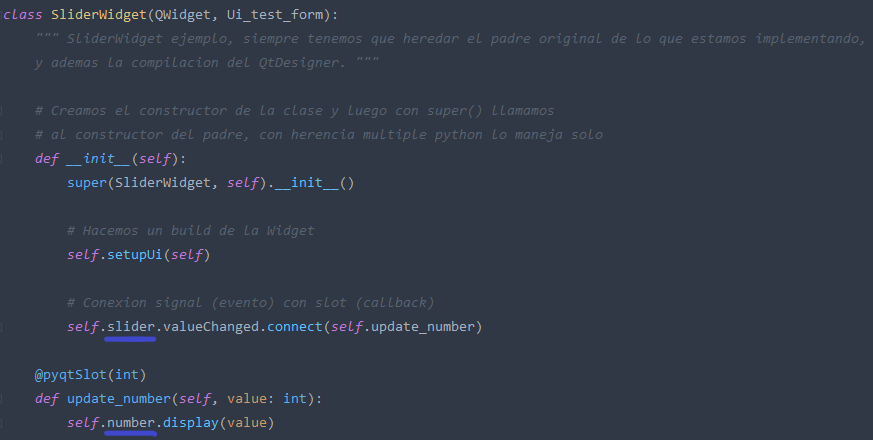
\includegraphics[scale=0.4]{imagenes/qtdesigner/qt_object_inspector_3.png}
    \end{tabular}
    \caption{Object Inspector de QtDesigner}
    \label{fig:qt_object_inspector}
\end{figure}

\subsubsection{Property Editor}
Cada uno de los objetos que pertenecen al \'arbol que muestra el Object Inspector, esta construido con un conjunto de clases a trav\'es del uso de un 
patr\'on de dise\~no de composici\'on. Lo importante es que podemos editar propiedades o atributos de cada una de esas partes que componen a nuestro objeto.

\begin{figure}[H]
    \centering
    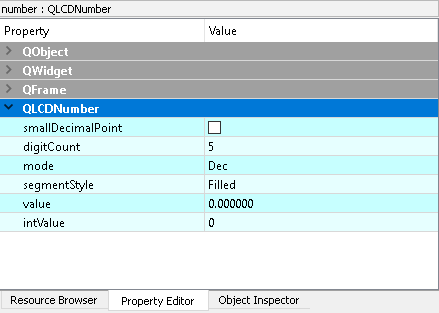
\includegraphics[scale=0.7]{imagenes/qtdesigner/qt_property_editor.PNG}
    \caption{Property Editor de QtDesigner}
    \label{fig:qt_property_editor}
\end{figure}

\subsubsection{Resource Browser}
El Resource Browser es muy importante, b\'asicamente para poder crear una ventana en la cual queremos incorportar contenido personalizado, sean imagenes,
audio o videos, e incluso archivos... es necesario crear lo que se define como un \textbf{Resource}. Cuando lo creamos, internamente podemos crear subcarpetas
para clasificar el contenido, por ejemplo, si queremos usar algunas imagenes para un bot\'on y otras para otro bot\'on, de esta forma cuando queramos utilizarlas estar\'an
disponibles.

\begin{figure}[H]
    \centering
    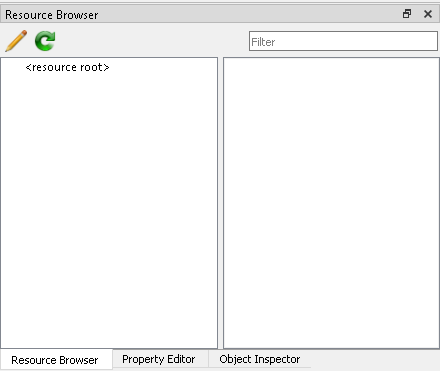
\includegraphics[scale=0.7]{imagenes/qtdesigner/qt_resource_browser_0.PNG}de
    \caption{Resource Browser: Ventana de recursos, apretando el lapiz las administramos}
    \label{fig:qt_resources_0}
\end{figure}

\begin{figure}[H]
    \centering
    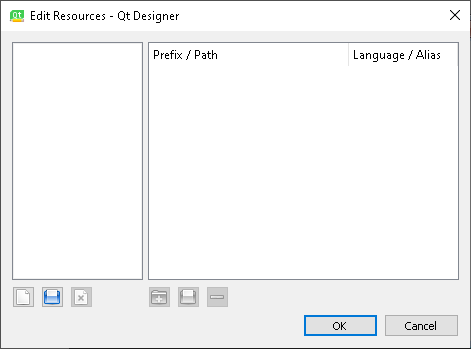
\includegraphics[scale=0.7]{imagenes/qtdesigner/qt_resource_browser_1.PNG}de
    \caption{Resource Browser: Con la hoja abajo a la izquierda creamos nuevos recursos.}
    \label{fig:qt_resources_1}
\end{figure}

\begin{figure}[H]
    \centering
    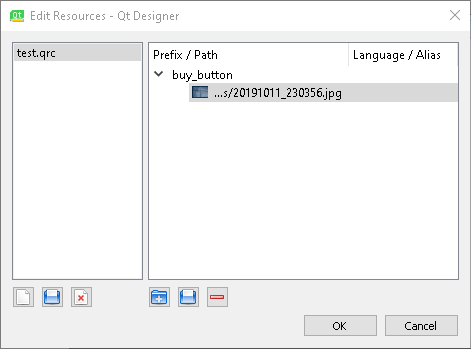
\includegraphics[scale=0.7]{imagenes/qtdesigner/qt_resource_browser_2.PNG}de
    \caption{Resource Browser: Agregamos Paths y sus contenidos}
    \label{fig:qt_resources_2}
\end{figure}

En primer lugar, ten\'e en cuenta que esto genera un archivo que seg\'un el ejemplo se llama \textbf{"test.qrc"}, este mismo
va a tener que ser compilado al igual que el dise\~no de la interfaz. Esto \'ultimo ser\'a explicado m\'as adelante.

\subsubsection{Signal/Slot Editor}
La IDE de QtDesigner tiene 4 modos de funcionamiento para el dise\~no de la aplicaci\'on y siempre nos encontramos en el modo
de edici\'on de Widgets. Otro modo posible es el de edici\'on de Signal/Slots, de lo cual podes aprender qu\'e es en \nameref{signal_slot},
mientras tanto consideremos que son eventos y callbacks para poder conectar funcionalidades de la aplicaci\'on. Este proceso de conexi\'on se puede hacer por c\'odigo
siempre, pero a veces se puede hacer en el modo de edici\'on mencionado, usando el bot\'on de la barra de herramientas o con F4.

En la Fig. \ref{fig:qt_signal_slot_0} se puede ver que nos aparece en rojo los Widgets, seleccionamos uno y arrastramos hacia otro,
al conectarse nos permite elegir una Signal del primero con un Slot del seguno a ser ejecutado. En este caso puedo utilizar sliderMoved(int)
con display(int).

\begin{figure}[H]
    \centering
    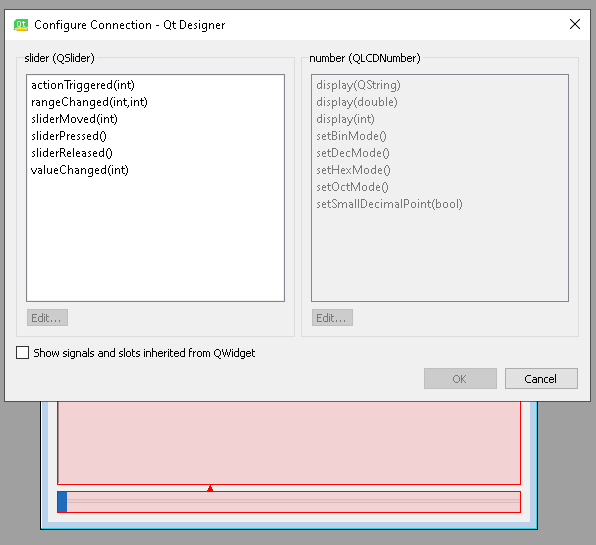
\includegraphics[scale=0.6]{imagenes/qtdesigner/qt_signal_slot_mode.PNG}
    \caption{Modo de edici\'on por Signal y Slot}
    \label{fig:qt_signal_slot_0}
\end{figure}

\begin{figure}[H]
    \centering
    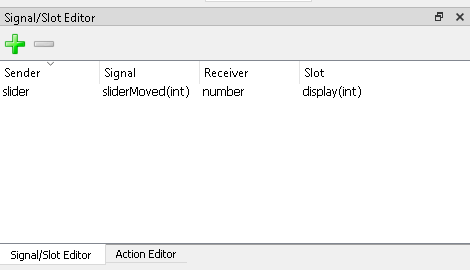
\includegraphics[scale=0.6]{imagenes/qtdesigner/qt_slot_singla.PNG}
    \caption{Ventana de conexiones de Signal y Slot}
    \label{fig:qt_signal_slot_1}
\end{figure}

\subsubsection{Action Editor}
En el dise\~no de aplicaciones de escritorio se usa mucho el concepto de Comandos, proveniente del patr\'on de dise\~no, donde lo que se busca es que una acci\'on
que es com\'unmente ejecutada por diversos eventos est\'e disponible de una forma distinta que un callback o slot. Eso es una QAction en PyQt.
Para que quede claro, la opci\'on Guardar, en una aplicaci\'on es un comando, y en PyQt se har\'ia como un QAction. De esta forma se puede vincular
para que sea disparada (.triggered()) por diferentes Widgets. S\'i, es casi lo mismo que un Slot.


Estas acciones pueden ser configuradas directamente en QtDesigner para que vincular que sean
ejecutadas por alg\'un evento dentro de la aplicaci\'on desde la IDE.

\subsection{Layouts y Containers: ¿Qu\'e son?}
Por el momento lo que deber\'iamos saber es que cuando creamos nuestro Form, sea QWidget, QDialog o QMainWindow, inicialmente vamos a poder
agregarle componentes a la GUI, no obstante cuando se lo crea por primera vez tales elementos quedan posicionados en ubicaciones \textbf{flotantes}.
Para garantizar que la aplicaci\'on quede bien ordenada, y que el motor de Qt sea capaz de hacer el build y el resize, es necesario utilizar Layouts y Containers.

\paragraph{Concepto clave:} Todo elemento de la GUI es un QWidget eventualmente, y todo QWidget puede albergar otros QWidgets, esto lo convierte en un container.

\paragraph{Layout:} Existen cuatro tipo de Layouts, b\'asicamente describen la forma en que se ordenan los Widgets dentro de un Widget. Puede ser \textbf{Vertical} u \textbf{Horizontal},
en tales casos se crea una pila de los Widgets en la orientaci\'on mencionada. Por otro lado est\'a \textbf{Grid} que los ordena por filas y columnas, y finalmente \textbf{Form}, que es un Grid
que siempre tiene dos columnas. El layout se configura f\'acilmente con la barra de herramientas o click derecho en el Widget.

\begin{figure}[H]
    \centering
    \begin{tabular}{c c}
        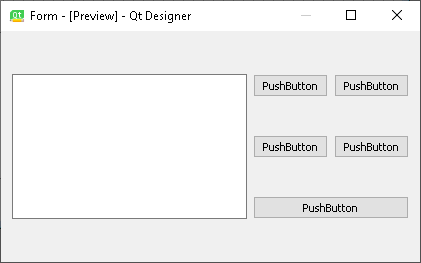
\includegraphics[scale=0.6]{imagenes/qtdesigner/qt_grid_layout.PNG} & 
        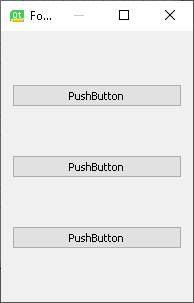
\includegraphics[scale=0.6]{imagenes/qtdesigner/qt_vertical_layout.PNG} \\ 
        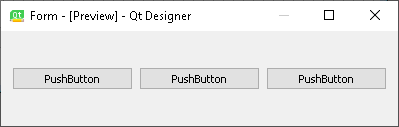
\includegraphics[scale=0.6]{imagenes/qtdesigner/qt_horizontal_layout.PNG} & 
        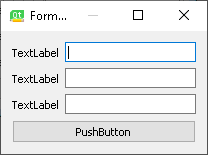
\includegraphics[scale=0.6]{imagenes/qtdesigner/qt_form_layout.PNG} 
    \end{tabular}
    \caption{Ejemplos de los Layouts}
\end{figure}

\paragraph{Containers:} Existen muchos tipos de containers, GroupBox, ScrollArea, ToolBox, TabWidget, StackedWidget, \'etc. La idea principal,
es que definen una forma caracter\'istica de contener otros Widgets, por ejemplo, cuando utilizamos StackedWidget podemos desplazarnos entre Widgets
como si fueran p\'aginas, a voluntad del usuario, o seg\'un lo programemos en Python.

\subsection{Paso a paso, ¿C\'omo creo una aplicaci\'on?}
Asumimos que lo que se explica en las otras partes sobre QtDesigner ya se ley\'o, y esto s\'olo explica los pasos generales a seguir
para llegar de principio a fin a nuestra aplicaci\'on ejecutable. Detalles sobre el dise\~no competen a otra secci\'on.

\begin{itemize}
    \item Creamos el Form que deseamos en QtDesigner. Sea QWidget, QDialog o QMainWindow.
    \item Agregamos los Widgets y definimos un Layout, organizamos nuestra GUI.
    \item Procuramos utilizar nombres representativos y bien definidos en el PropertyEditor.
    \item Guardamos el archivo en nuestra carpeta, al igual que los dem\'as archivos como Resources si usamos.
    \item Luego realizamos el proceso de compilaci\'on ejecutando los comandos, \nameref{compilar_design} y \nameref{compilar_recurso}.
    \item A partir de esto obtenemos nuestro archivo .py compilado.
\end{itemize}

Hasta este punto, se ilustran a continuaci\'on las figuras que describen estos pasos, as\'i como la estructura propuesta de archivos para ello,
que puede ser revisada en \nameref{estructura_programas}.

\begin{figure}[H]
    \centering
    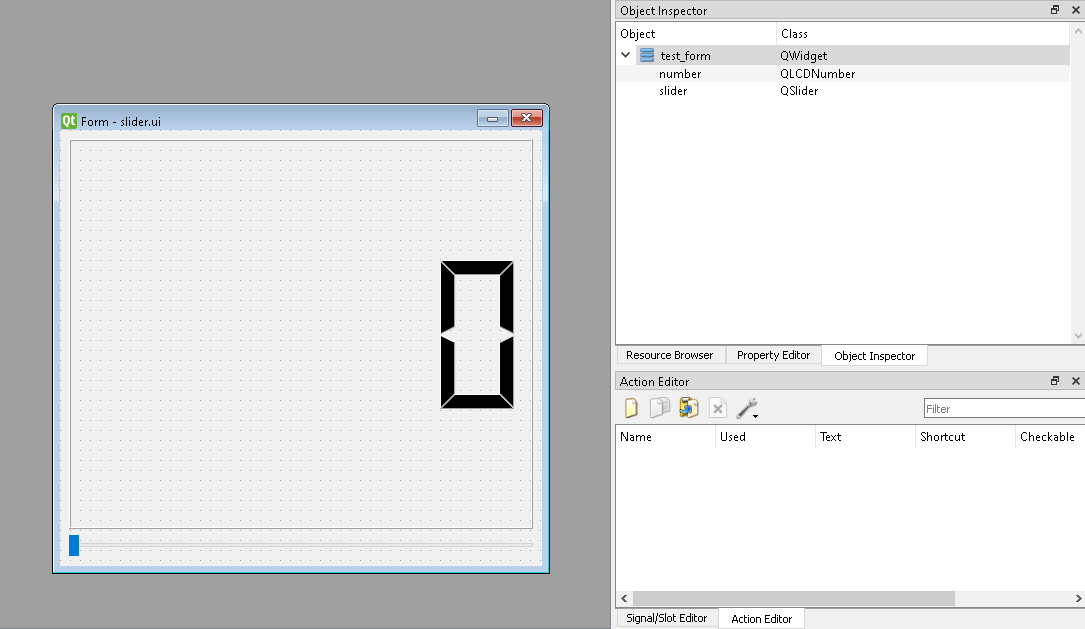
\includegraphics[scale=0.4]{imagenes/qtdesigner/qt_steps.PNG}
\end{figure}

\begin{figure}[H]
    \centering
    
\includegraphics[scale=0.7]{imagenes/qtdesigner/qt_steps_1.PNG}
\end{figure}

\begin{figure}[H]
    \centering
    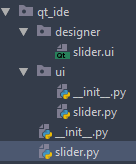
\includegraphics[scale=0.8]{imagenes/qtdesigner/qt_steps_2.PNG}
\end{figure}

En la carpeta designer coloco los archivos propios del QtDesigner, luego en "ui" los resultados de la compilaci\'on. Finalmente en un nivel superior de directorio,
creo un nuevo archivo slider.py en el cual crear\'e propiamente la clase, la construir\'e y luego realizar\'e las conexiones de la GUI con el backend de mi aplicaci\'on.

\begin{lstlisting}{language=Python}
# PyQt5 Modules
from PyQt5.QtWidgets import QApplication
from PyQt5.QtWidgets import QWidget

# Project Modules
from ui.slider import Ui_test_form


class Slider(QWidget, Ui_test_form):
    # Creamos nuestra clase Slider, hacemos que herede del resultado de la compilacion
    # y de su Padre original en este caso QWidget.

    def __init__(self):
        # Creamos el constructor y llamamos al constructor de los padres
        # luego utilizamos el metodo para la inicializacion de los widgets internos
        super(Slider, self).__init__()
        self.setupUi(self)


if __name__ == "__main__.py":
    # Contexto o aplicacion
    app = QApplication([])

    # Instancia para probar nuestra Widget
    widget = Slider()
    widget.show()

    # Loop de eventos de la app
    app.exec()

\end{lstlisting}

\subsection{BonusTrack: ¿Qu\'e cosas copadas tiene PyQt?}

\subsubsection{Ventanas de di\'alogo para reutilizar}
\label{dialogs_utiles}

Existen algunos di\'alogos ya creados por el framework de Qt para que reutilicemos,
como el \textbf{QFileDialog}, \textbf{QMessageBox}, \textbf{QColorDialog}, \textbf{QInputDialog}, \textbf{QProgressDialog},
entre otros... y su utilizaci\'on es muy sencilla. Observar en la Fig. \ref{fig:qt_dialog_examples}.

Se los puede utilizar configurandolos con el constructor, instanci\'andolos y luego llamando a alguno de sus m\'etodos para hacerlos
visibles y luego recuperar los datos que obtuvieron. Por otro lado, se pueden ejecutar desde alguno de sus m\'etodos est\'aticos.

\begin{figure}[H]
    \centering
    \begin{tabular}{c c}
        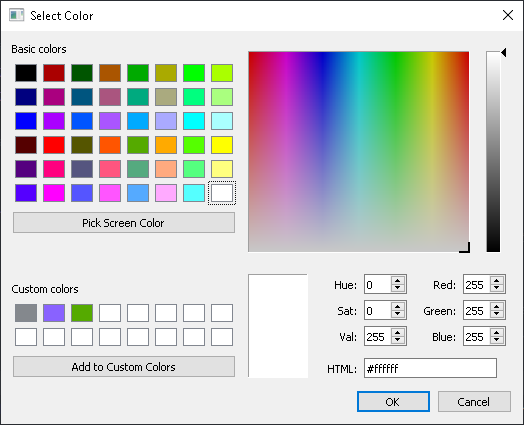
\includegraphics[scale=0.4]{imagenes/qtdesigner/qt_color_dialog.PNG} &
        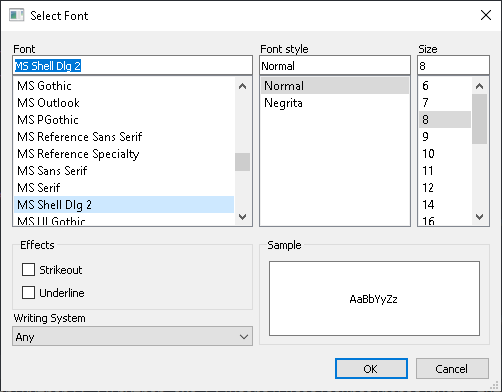
\includegraphics[scale=0.5]{imagenes/qtdesigner/qt_font_dialog.PNG} \\
        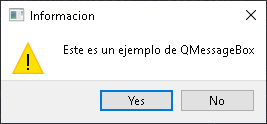
\includegraphics[scale=0.6]{imagenes/qtdesigner/qt_message_dialog.PNG} &
        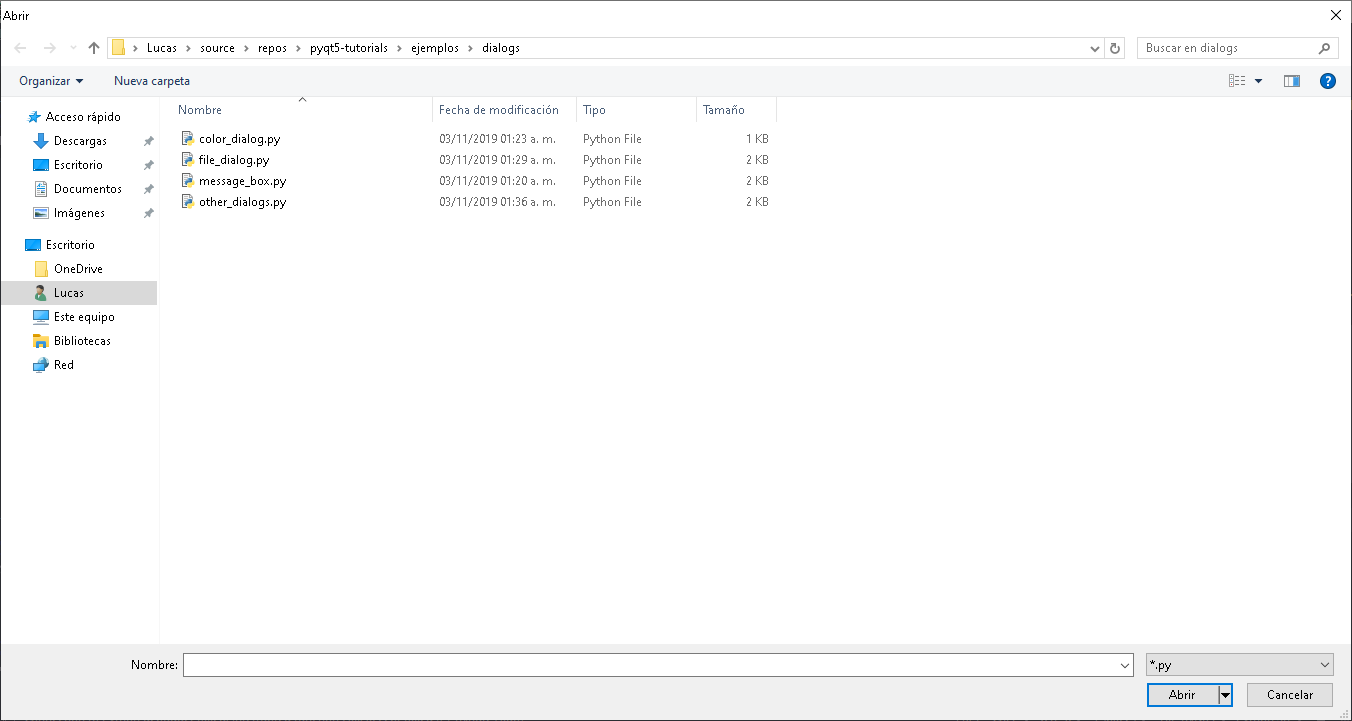
\includegraphics[scale=0.2]{imagenes/qtdesigner/qt_file_dialog.PNG} 
    \end{tabular}
    \caption{Ejemplos de QColorDialog, QFileDialog, QFontDialog y QMessageBox}
    \label{fig:qt_dialog_examples}
\end{figure}

